\section{Plano de integração e validação} % (fold)
\label{sec:plano_de_integração_e_validação}
	Com os subsistemas devidamente projetados, tenstados e operantes, é preciso estabeler planos de integração desses subsistemas para garantir que não haja falhas durante esse processo, alem disso é preciso propor testes de validação para cada plano estabelecido.

	Os planos de integração e os testes de validação foram elaborados pelos subgrupos responsáveis por cada subsistema, dessa forma os planos serão dispostos evidenciando separadamente os subsistemas.

	\subsection{Alimentação}
	\label{sub:plano_alimentação}

	\subsection{Comunicação}
	\label{sub:plano_comunicação}

	\subsection{Estrutura da Base}
	\label{sub:plano_estrutura}

	\subsection{Estrutura e Locomoção}
	\label{sub:plano_locomoção}

	\subsection{Interface}
	\label{sub:plano_interface}

	\subsection{Navegação}
	\label{sub:plano_navegação}

	\subsection{Sensoriamento}
	\label{sub:plano_sensoriamento}
		A figura \ref{img:planejamento_robo} apresenta um esquemático elaborado pela equipe de eletrônica para definir as relações que devem ser estabelecidas entre os componentes para que o mesmo funcione corretamente.

		\begin{figure}[H]                                                           
      		\centering                                                                
      		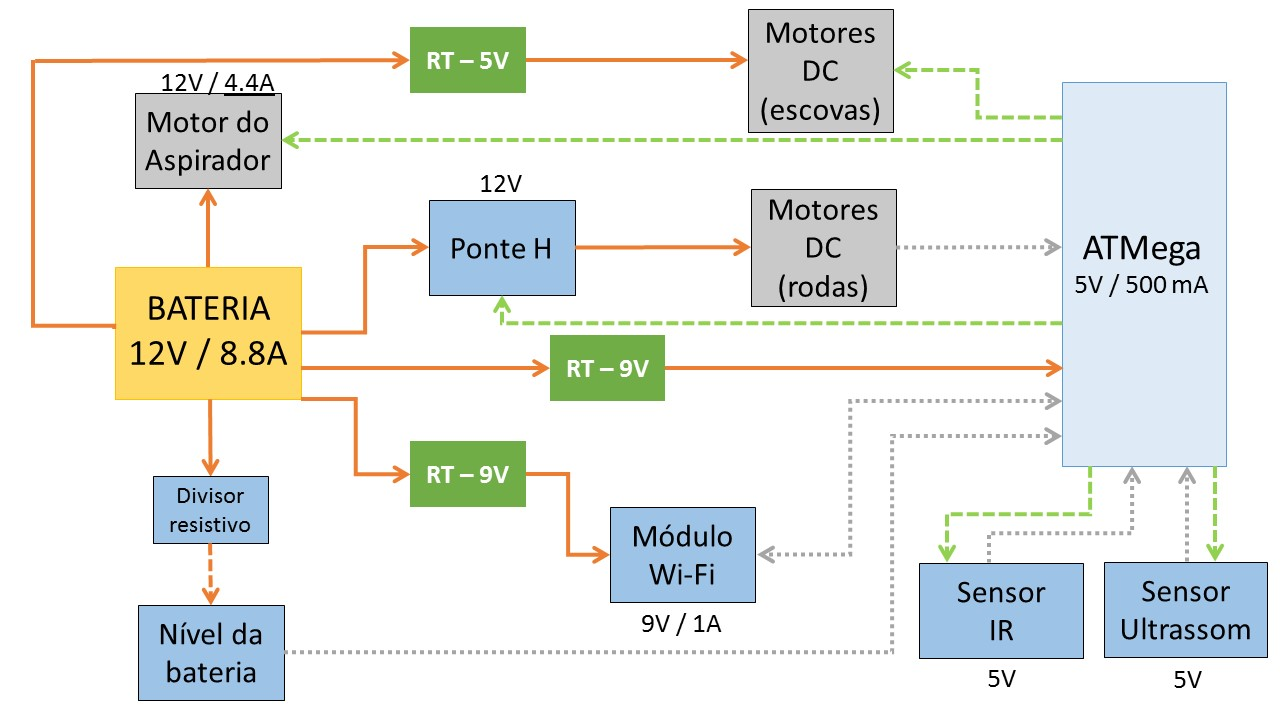
\includegraphics[scale=0.5]{figuras/Planejamento_robo.jpg}               
      		\caption{Esquemático elaborado para definir os tipos de relações entre existentes entre os sistemas. \textbf{Legenda}: Setas Laranjas: alimentação ; Setas Verdes: controle ; Setas Cinzas: comunicação}    
      		\label{img:planejamento_robo}                                            
    	\end{figure} 

    	Começando pela bateria de 12 volts que é a fonte de alimentação do aspirador e alimentará paralelamente o motor do sistema de sucção, a ponte H, os motores das escovas de limpeza, o módulo wi-fi, o sensor de bateria e o controlador ATMEga. A tensão de alimentação de cada um desses dispositivos é diferente, por isso será necessário utilizar reguladores com faixas de tensão variadas para que todos os componentes operem na sua faixa de tensão ideal.

    	Os motores DC das escovas de limpezas serão controlados por meio de transistores chaveados que receberão sinais do ATMEga de acordo com a interface com o usuário. A ponte H alimenta os motores das rodas e por meio de sinais PWM que recebe do ATMega, controla a direção de rotação e velocidade dos motores. O módulo wi-fi manda para o ATMega informações sobre a potência do sinal recebido. E os sensores ultrassônicos e IR recebem sinais do controlador e retornam para ele a distância em que se encontram os obstáculos. Por fim o sensor de tensão monitora constantemente o nível de tensão da bateria e envia para o controlador a informação sobre quando a carga está muito baixa.

    	Do ponto de vista da integração, o aspirador será ativado por meio de uma interface com o usuário, essa ativação iniciará o movimento dos motores e do sistema de sucção. Com o monitoramento constante dos sensores o aspirador andará pelo cômodo, através do algoritmo de navegação que será implementado, desviando de obstáculos pelo caminho e realizando a limpeza do cômodo. Quando a bateria estiver fraca ou quando a limpeza do cômodo for completada, o módulo será ativado e medirá a potência do sinal wi-fi para que o aspirador saiba onde se encontra a base, ele então irá se dirigir para a direção onde a potência é mais forte. Por fim chegando a base, a bateria será recarregada e o aspirador permanecerá no lugar até que a próxima limpeza seja agendada.  

	\subsection{Sucção}
	\label{sub:plano_sucção}


% section plano_de_integração_e_validação (end)